\section{Compiler Implementation}\label{sec:compiler}



%-----------------------------------------------------------------------------
\subsection{Omni XMP Compiler Framework}
%-----------------------------------------------------------------------------

\begin{figure}[tbh]
 \begin{center}
  % trimはleft bottom right topの順
  %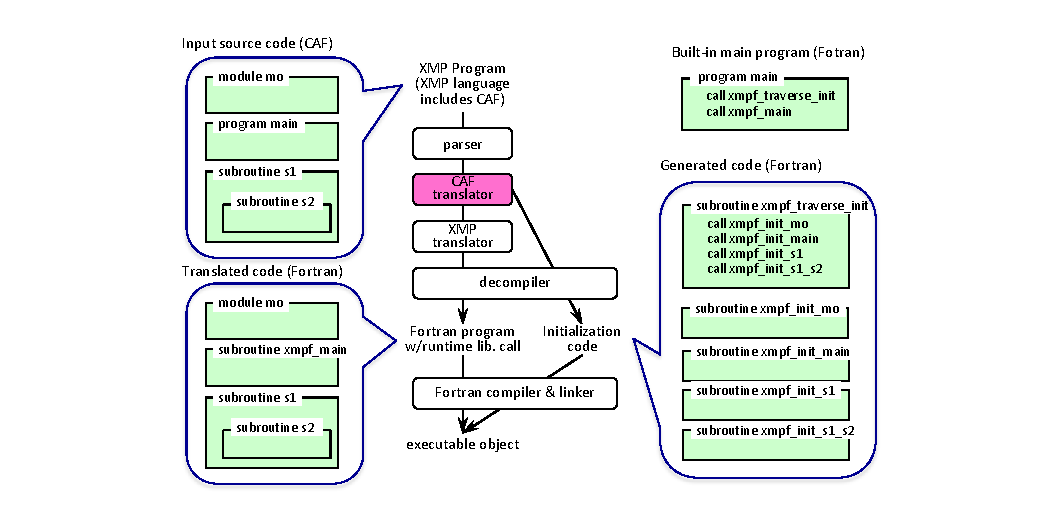
\includegraphics[scale=0.55,trim=6cm 0cm 4cm 6cm,clip]{figs/translator-tmp.pdf}
  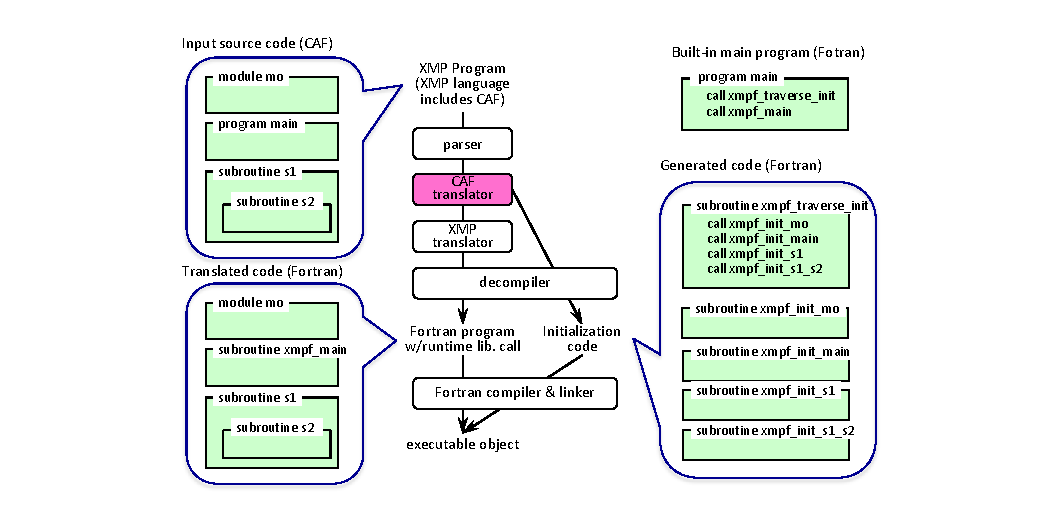
\includegraphics[trim=30mm 0mm 20mm 7mm, scale=1.0]{figs/translator-tmp.pdf}
  \caption{XMP compiler and an example of coarray program compilation}
  \label{fig:translator}
  %-- 修正すべき箇所
  CAF translator $\rightarrow$ coarray translator
 \end{center}
\end{figure}

The CAF translator was added into the Omni XMP compiler as shown in Figure~\ref{fig:translator}.
The Omni XMP compiler is a source-to-source translator that converts XMP programs into 
the base language (Fortran or C).  The component `coarray translator' is located in 
front of the XMP translator to solve coarray features previously. The output of the decompiler 
is a standard Fortran/C program that may include calls to the XMP runtime library.

To initialize static coarray variables prior to the execution of the user program, 
the built-in main program is made in order to call the initialization routine 
{\tt xmpf\_traverse\_init} followed by user’s main program.
{\tt xmpf\_traverse\_init} is generated by the coarray translator to call initialization 
routines (e.x., {\tt xmpf\_init\_foo}) corresponding to user-defined procedures (e.x., {\tt foo}).

initializationの内容は以下の通り
\begin{itemize}
\item
プログラム全体の宣言文から個々のstatic coarray変数のサイズ(バイト数)を算出。
名前付き定数や簡単な演算、組み込み関数を含む定数式評価で求める。
\item
領域を通信ライブラリにregisterする。
CA (Compiler Allocation) methodでは、領域の割付けはコンパイラ処理系に任せて、
結果のアドレスを通信ライブラリに登録する。
RA (Runtime-library Allocation) methodでは、
通信ライブラリに必要なサイズを与えて領域割付けと登録を同時に行う。
\end{itemize}

Figure~\ref{fig:register-RA-CA} illustrates the memory allocation and registration
on RA and CA methods. 
Because the allocated memory address is decided in the runtime library in the RA
method, the user object code must accept the address allocated 
inside the runtime system as an address of a regal Fortran variable.
To make this connection, it was necessary to use the Cray pointer, which is not 
in the Fortran standard.
In the case of the CA method, the runtime library accepts the address allocated
in the Fortran system, and registers to the communication library.

\begin{figure}[tbh]
 \begin{center}
  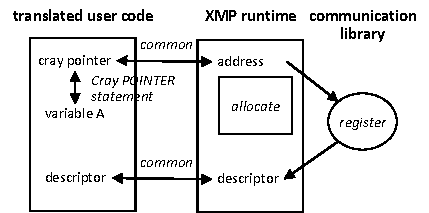
\includegraphics[scale=0.9, trim=0mm 0mm 0mm 0mm, clip]{figs/register-RA-tmp.pdf}\\
The runtime allocates and registers coarrays and passes the address to the user code.
 \end{center}
 \begin{center}
(a) RA method
 \end{center}
 \begin{center}
  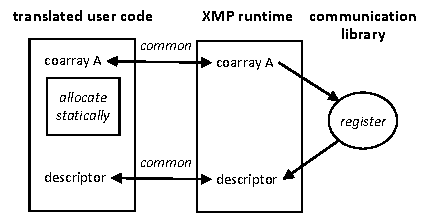
\includegraphics[scale=0.9, trim=0mm 0mm 0mm 0mm, clip]{figs/register-CA-tmp.pdf}\\
The user code allocates coarrays and causes the runtime to register with the address.
 \end{center}
 \begin{center}
(b) CA method
 \end{center}
 \caption{Memory allocation for coarrays in RA and CA methods}
 \label{fig:register-RA-CA}
\end{figure}


%-----------------------------------------------------------------------------
\subsection{PUT/GET Communication}
%-----------------------------------------------------------------------------

To avoid disturbing the execution on the remote image, PUT and GET communications
are implemented always using Remote Direct Memory Access (RDMA) provided by 
the communication library (except coarrays with pointer/allocatable structure components). 
In contrast, local data access is selective between using Direct Memory Access (DMA) or
using a local buffer. For the buffer scheme, one of four algorithms will be chosen 
depending on three parameters, the size of the local buffer $B$ and the 
local and remote contiguous lengths $N_L$ and $N_R$.
$B$ should be large enough to ignore communication latency overhead and we use
about 400 kilo-bites in default. Unlike the case of MPI message passing,
coarray PUT/GET communication requires only one local buffer for any numbers of
other images.
$N_L$ and $N_R$ can be evaluated at runtime. The Fortran syntax guarantees 
that $N_L$ is a multiple of $N_R$ or $N_R$ is a multiple of $N_L$.
An algorithm to get the contiguous length is shown in the paper~\cite{pgas15}.

Table~\ref{tab:putget} summarizes our algorithm for PUT/GET communication for five cases.
The unit size is the chunk length of the PUT/GET communication.
Case~0 shows the algorithm using RDMA-DMA PUT/GET communication and Cases~1 through~4
shows the algorithms using RDMA and local-buffering. 
Due to its strict condition, the DMA scheme is rarely used.
And it is not always faster than the buffering scheme cases~2 and~3 because of the 
difference of the unit sizes. The merit of cases~2 and~3 is that the unit size 
is extended to a multiple of $N_L$ by gathering number of short contiguous data in the buffer,
or by scattering from the buffer into number of short contiguous data.

\begin{table}[tbh]
 \caption{Summary of the PUT/GET algorithm related to $N_L$, $N_R$ and $B$}
 \label{tab:putget}
 \begin{flushleft}
  \begin{tabular}{|@{~}c@{~}|c||@{~}c@{~}|@{~}c@{~}|}
\hline
scheme &
case &
condition &
unit size \\
\hline
\hline
DMA &
&
Local data is registered. &
$\min(N_L, N_R)$ \\
\hline
buffering &
1 & 
$N_R \leq B,~ N_R \leq N_L$ &
$N_R$ \\
\cline{2-4}
&
2 &
$N_L < N_R \leq B$ &
$N_R$ \\
\cline{2-4}
&
3 &
$N_L < B < N_R$ &
multiple of $N_L$ ($\leq B$) \\
\cline{2-4}
&
4 &
$B < N_R,~ B \leq N_L$ &
$B$ (or less than $B$ at last) \\
\hline
  \end{tabular}
 \end{flushleft}
 \begin{flushleft}
  \begin{tabular}{|@{~}c@{~}|c||@{~~}l@{~~}|@{~~}l@{~~}|}
\hline
scheme &
case &
PUT action for every unit &
GET action for every unit \\
\hline
\hline
DMA &
&
put once &
get once \\
\hline
buffering &
1 &
buffer once and put once &
get once and unbuffer once \\
\cline{2-4}
&
2 &
buffer for each $N_L$, and put once &
get once, and unbuffer for each $N_L$ \\
\cline{2-4}
&
3 &
buffer for each $N_L$, and put once &
get once, and unbuffer for each $N_L$ \\
\cline{2-4}
&
4 &
buffer once and put once &
get once and unbuffer once \\
\hline
  \end{tabular}
 \end{flushleft}
\end{table}



%-----------------------------------------------------------------------------
\subsection{Nonblocking communication}
%-----------------------------------------------------------------------------





